%% ============================================================
%%  SECCIÓN 5 — Materiales y Equipos
%% ============================================================

\section{Materiales y Equipos}
\label{sec:materiales}

Para el desarrollo experimental de la práctica en la Mesa C7 se utilizaron instrumentos de generación de señal, adquisición digital de datos y componentes pasivos patronados. A continuación se detallan sus características técnicas, funciones y especificaciones metrológicas.

\subsection{Osciloscopio Digital Rohde \& Schwarz HMO1202}
\begin{itemize}
    \item \textbf{Descripción y función:} Instrumento digital de adquisición y visualización en tiempo real de dos canales analógicos independientes (CH1 y CH2). Se utilizó para registrar simultáneamente la curva de carga/descarga en el condensador ($V_C(t)$ en CH1) y la caída en la resistencia ($V_R(t)$ en CH2), así como para realizar mediciones temporales mediante cursores digitales y suma matemática de señales (\texttt{MATH ADD}) \cite{hmo1202}, tal como se ilustra en la Fig.~\ref{fig:mat_osciloscopio}.
    \item \textbf{Especificaciones técnicas:} Ancho de banda de \qty{200}{\mega\hertz}, tasa de muestreo máxima de \qty{2}{\giga\sample\per\second}, memoria de adquisición de 2 Mpts por canal, pantalla TFT color de \qty{6,5}{\inch} con resolución VGA ($640 \times 480$ píxeles) y estabilidad de base de tiempo de \qty{50}{\ppm}.
    \item \textbf{Incertidumbre instrumental:} En la escala de deflexión vertical (\qtyrange{1}{5}{\volt\per\division}), la precisión en ganancia DC es de $\pm\qty{2}{\percent}$ del fondo de escala; la resolución en la lectura de tiempo con cursores en pantalla es de $\delta t = \qty{0,1}{\micro\second}$, con una incertidumbre combinada evaluada en $u(\tau) \approx \qty{0,14}{\micro\second}$ \cite{gum}.
    \item \textbf{Precauciones operativas:} Establecer una referencia de tierra común obligatoria entre ambos canales conectando los cocodrilos negros de las sondas al nodo central de unión entre el resistor y el capacitor, evitando lazos de masa cortocircuitantes.
\end{itemize}

\begin{figure}[H]
    \centering
    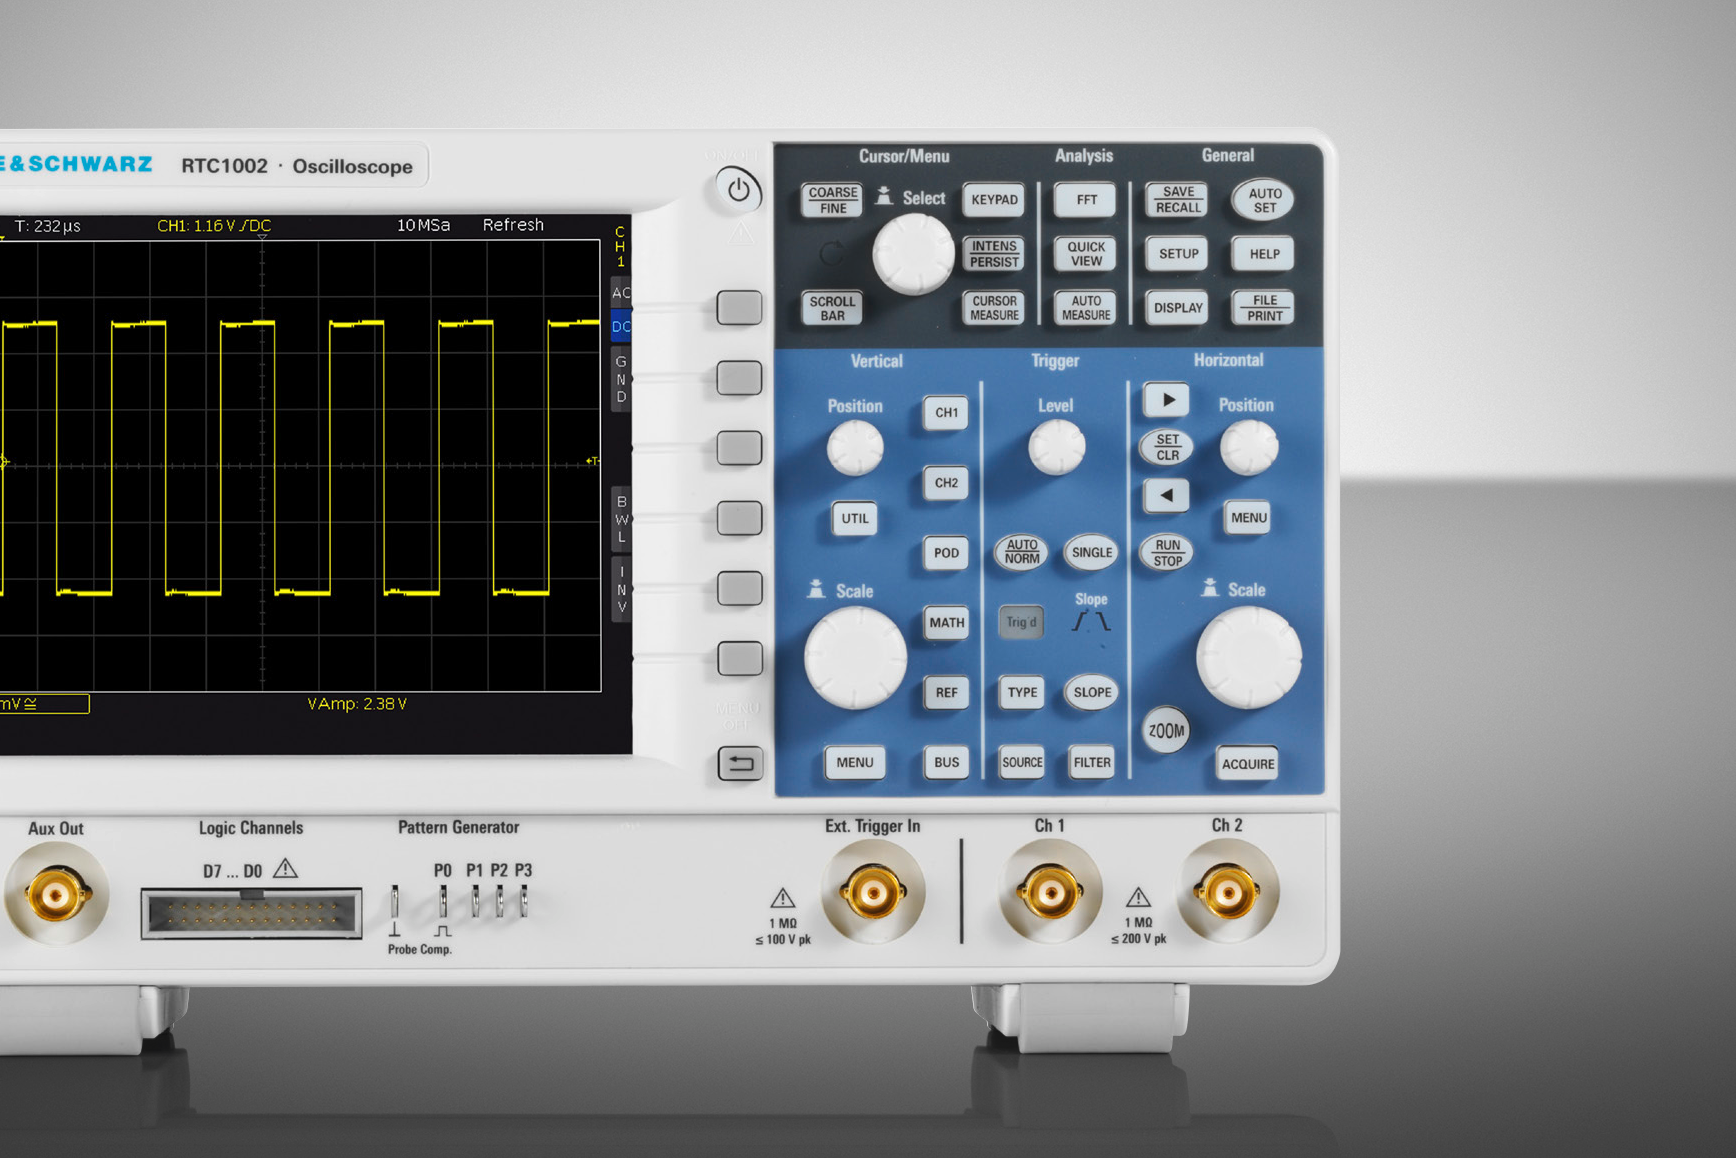
\includegraphics[width=0.50\linewidth, height=5.5cm]{fig_osciloscopio}
    \caption{Osciloscopio digital Rohde \& Schwarz HMO1202 empleado para la captura y medición de señales transitorias.}
    \label{fig:mat_osciloscopio}
\end{figure}

\subsection{Generador de Funciones Arbitrario OWON AG 051F}
\begin{itemize}
    \item \textbf{Descripción y función:} Fuente sintetizadora de señales basada en tecnología de síntesis digital directa (DDS). Suministró la excitación periódica de onda cuadrada al circuito RC, operando como un conmutador de dos niveles de potencial continuo (\qty{10,0}{\voltpp} y \qty{0}{\volt}) \cite{owon_ag} (ver Fig.~\ref{fig:mat_generador}).
    \item \textbf{Especificaciones técnicas:} Rango de frecuencia hasta \qty{50}{\mega\hertz}, resolución en frecuencia de \qty{1}{\micro\hertz}, estabilidad térmica de $\pm\qty{1}{\ppm}$, impedancia de salida nominal de \qty{50}{\ohm} y distorsión armónica total menor a $\qty{0,2}{\percent}$.
    \item \textbf{Condición de operación:} Frecuencia fijada en $f = \qty{250}{\hertz}$ (semiperíodo $T/2 = \qty{2,00}{\milli\second}$), amplitud calibrada en \qty{10,0}{\voltpp} (amplitud pico de \qty{5,0}{\volt} con desplazamiento offset de $+5{,}0\ \unit{\volt}$ para oscilar entre \qty{0}{\volt} y \qty{10,0}{\volt}) y ciclo de trabajo del \qty{50}{\percent}.
    \item \textbf{Precauciones operativas:} Verificar la correcta adaptación de impedancia en la pantalla del instrumento (ajustada a alta impedancia \texttt{High-Z}) para que la amplitud leída en el menú coincida con el voltaje real suministrado al circuito.
\end{itemize}

\begin{figure}[H]
    \centering
    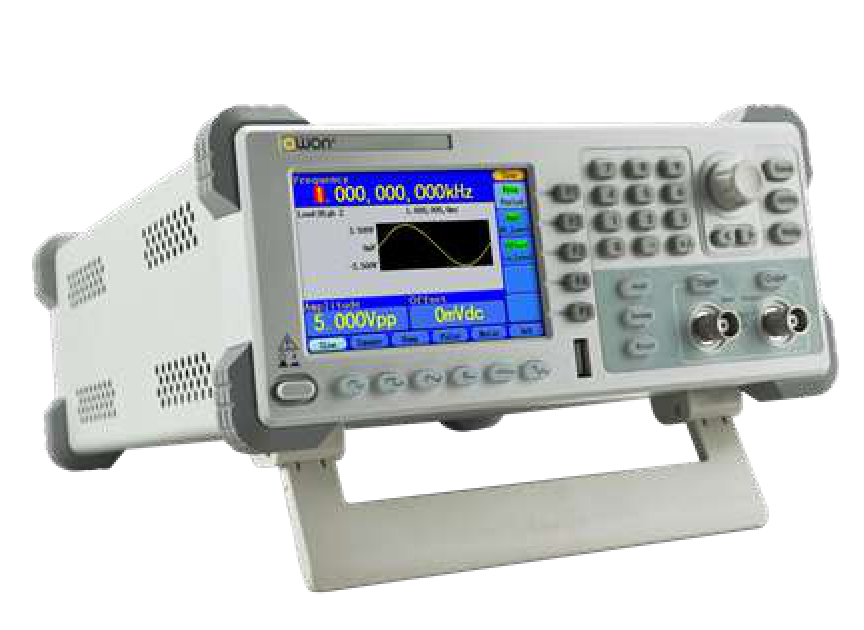
\includegraphics[width=0.50\linewidth, height=5.5cm]{fig_generador}
    \caption{Generador de funciones arbitrario OWON AG 051F utilizado como fuente de excitación cuadrada periódica.}
    \label{fig:mat_generador}
\end{figure}

\subsection{Multímetro Digital Portátil}
\begin{itemize}
    \item \textbf{Descripción y función:} Instrumento multifunción de $3\frac{1}{2}$ dígitos empleado en modo óhmetro de precisión para medir previamente los valores reales de resistencia de los resistores de película metálica asignados a la Mesa C7 (ver Fig.~\ref{fig:mat_multimetro}).
    \item \textbf{Especificaciones y tolerancia:} En la escala de \qty{20}{\kilo\ohm}, resolución de visualización de \qty{0,01}{\kilo\ohm} (\qty{10}{\ohm}) y tolerancia de fabricante de $\pm(\qty{0,8}{\percent}\,\text{lectura} + 2\text{ dígitos})$. En la escala de \qty{2}{\kilo\ohm}, resolución de \qty{0,001}{\kilo\ohm} (\qty{1}{\ohm}) y tolerancia de $\pm(\qty{0,8}{\percent}\,\text{lectura} + 2\text{ dígitos})$.
    \item \textbf{Incertidumbres Tipo B calculadas (GUM):} Para $R_1 = \qty{9980}{\ohm}$, $u(R_1) = \qty{57,6}{\ohm}$; para $R_2 = \qty{6832}{\ohm}$, $u(R_2) = \qty{32,7}{\ohm}$; para $R_3 = \qty{2250}{\ohm}$, $u(R_3) = \qty{11,5}{\ohm}$.
    \item \textbf{Precauciones operativas:} Medir las resistencias completamente desconectadas del circuito para impedir derivaciones de corriente a través de otros elementos de la placa.
\end{itemize}

\begin{figure}[H]
    \centering
    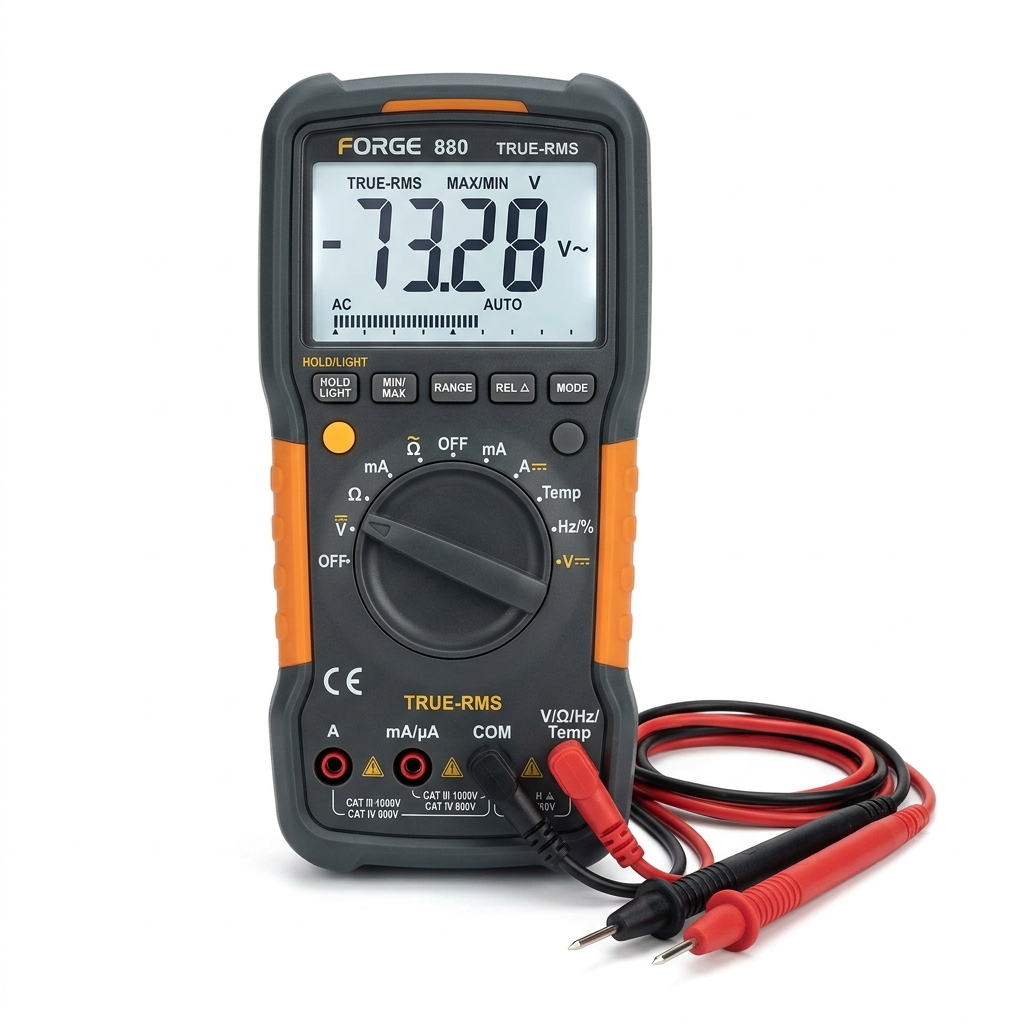
\includegraphics[width=0.50\linewidth, height=5.5cm]{fig_multimetro}
    \caption{Multímetro digital portátil empleado para la caracterización ohmimétrica de los resistores de banco.}
    \label{fig:mat_multimetro}
\end{figure}

\subsection{Módulo Acrílico de Componentes RC de Laboratorio}
\begin{itemize}
    \item \textbf{Descripción y componentes:} Placa experimental acrílica provista de bornes de conexión rápida tipo banana de \qty{4}{\milli\meter} (ver Fig.~\ref{fig:mat_caja_elementos}), equipada con tres resistencias de precisión y tres condensadores rotulados:
    \begin{itemize}
        \item Resistencia $R_1$: nominal de \qty{10}{\kilo\ohm}, valor medido en Mesa C7: \qty{9,980 \pm 0,058}{\kilo\ohm}.
        \item Resistencia $R_2$: nominal de \qty{6,8}{\kilo\ohm}, valor medido en Mesa C7: \qty{6,832 \pm 0,033}{\kilo\ohm}.
        \item Resistencia $R_3$: nominal de \qty{2,2}{\kilo\ohm}, valor medido en Mesa C7: \qty{2,250 \pm 0,012}{\kilo\ohm}.
        \item Condensador $C_1$: valor rotulado en el módulo: \qty{10,0}{\nano\farad} (\qty{0,01}{\micro\farad}).
        \item Condensador $C_2$: valor rotulado en el módulo: \qty{22,40}{\nano\farad} (\qty{0,02240}{\micro\farad}).
        \item Condensador $C_3$: valor rotulado en el módulo: \qty{33,23}{\nano\farad}.
    \end{itemize}
    \item \textbf{Aclaración metrológica sobre unidades:} Aunque las etiquetas históricas del módulo emplean en ocasiones el prefijo microfaradio (\unit{\micro\farad}), los valores numéricos ($10{,}0$, $22{,}40$, $33{,}23$) corresponden estrictamente a nanofaradios (\unit{\nano\farad}), tal como se demostró físicamente en el plan de trabajo para compatibilizar la constante de tiempo con el semiperíodo de excitación de \qty{2,00}{\milli\second}.
\end{itemize}

\begin{figure}[H]
    \centering
    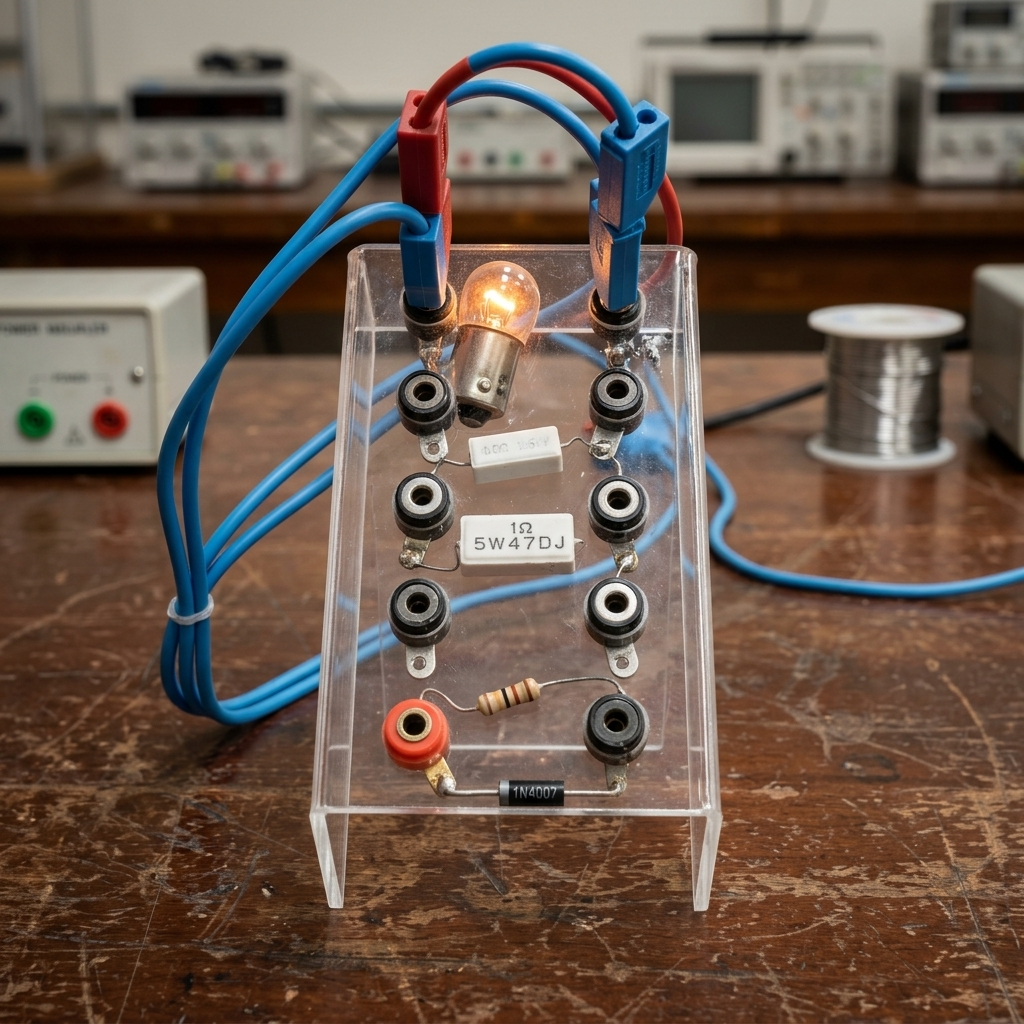
\includegraphics[width=0.50\linewidth, height=5.5cm]{fig_caja_elementos}
    \caption{Módulo didáctico de laboratorio con bornes de acoplamiento rápido para resistores y capacitores.}
    \label{fig:mat_caja_elementos}
\end{figure}

\subsection{Cables Coaxiales BNC, Sondas y Puentes de Conexión}
\begin{itemize}
    \item \textbf{Descripción:} Dos cables coaxiales de \qty{50}{\ohm} blindados (tipo RG-58) provistos de conector BNC en un extremo y pinzas cocodrilo en el opuesto para la inyección de señal y toma de datos; cables flexibles con conectores banana macho-macho apilables para el conexionado inter-módulos (ver Fig.~\ref{fig:mat_cables_sondas}).
    \item \textbf{Efectos parásitos:} Resistencia óhmica de contacto inferior a \qty{0,05}{\ohm} y capacitancia parásita de cable de aproximadamente \qty{30}{\pico\farad\per\meter}, despreciable frente a los \qty{10}{\nano\farad} mínimos de los condensadores bajo estudio.
\end{itemize}

\begin{figure}[H]
    \centering
    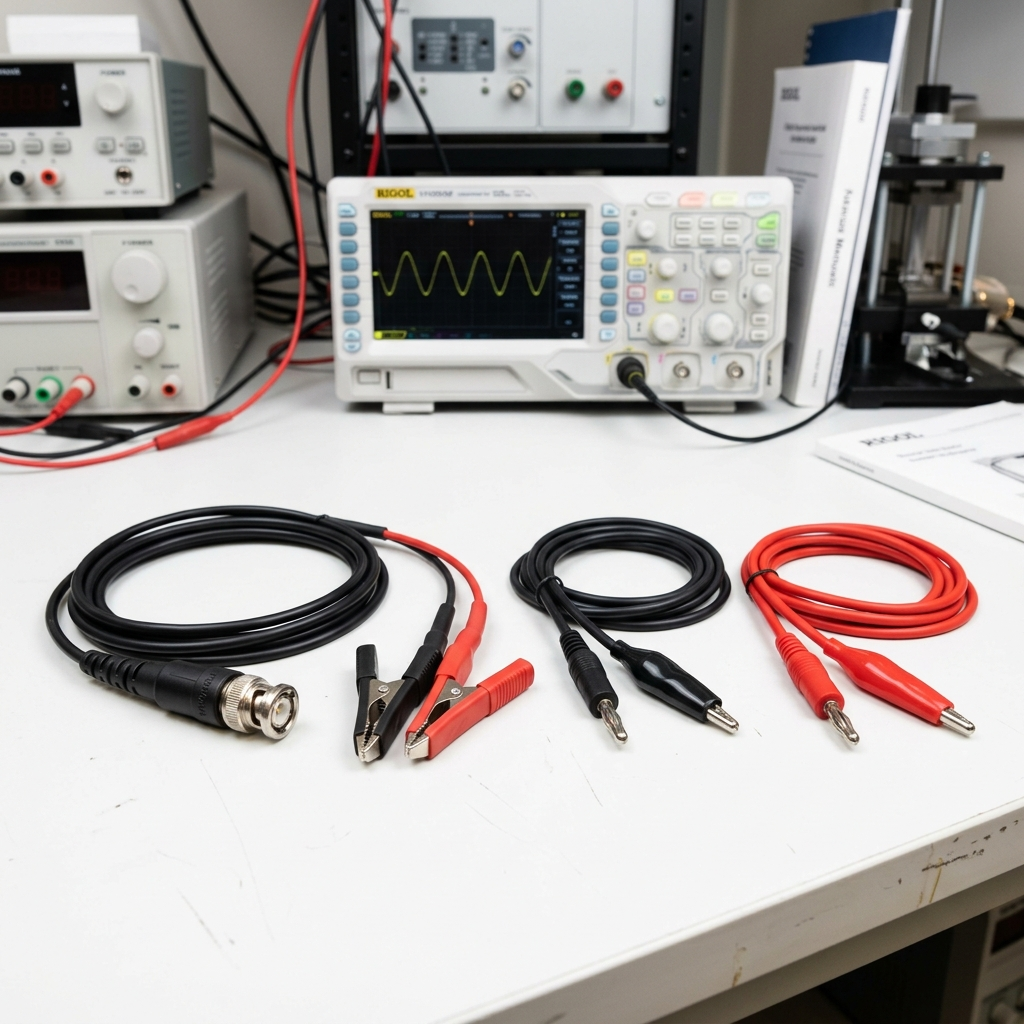
\includegraphics[width=0.50\linewidth, height=5.5cm]{fig_cables_sondas}
    \caption{Conjunto de cables coaxiales BNC-caimán y terminales banana empleados para el cableado de la red.}
    \label{fig:mat_cables_sondas}
\end{figure}

En la Tabla~\ref{tab:especificaciones_equipos} se resumen las características metrológicas de los principales equipos e instrumentos empleados en la sesión práctica.

\begin{table}[H]
    \centering
    \caption{Especificaciones metrológicas e incertidumbres instrumentales de los equipos utilizados.}
    \label{tab:especificaciones_equipos}
    \resizebox{\linewidth}{!}{%
    \begin{tabular}{lcccc}
        \toprule
        \textbf{Instrumento / Equipo} & \textbf{Modelo} & \textbf{Rango Operativo} & \textbf{Resolución} & \textbf{Incertidumbre Instrumental} \\
        \midrule
        Osciloscopio Digital & Rohde \& Schwarz HMO1202 & \qtyrange{1}{10}{\voltpp} & \qty{0,1}{\micro\second} & $\pm(\qty{2}{\percent}\,\text{ganancia} + \qty{0,14}{\micro\second}\,\text{tiempo})$ \\
        Generador de Funciones & OWON AG 051F & \qty{1}{\micro\hertz} -- \qty{50}{\mega\hertz} & \qty{1}{\micro\hertz} & $\pm\qty{1}{\ppm}$ en frecuencia \\
        Multímetro Digital & Portátil $3\frac{1}{2}$ dgt & \qtyrange{0,2}{20}{\kilo\ohm} & \qty{1}{\ohm} -- \qty{10}{\ohm} & $\pm(\qty{0,8}{\percent}\,\text{lectura} + 2\text{ dgt})$ \\
        Resistencias de Película & Placa de pruebas & \qtyrange{2,2}{10}{\kilo\ohm} & --- & Tolerancia nominal de fábrica $\pm\qty{5}{\percent}$ \\
        Condensadores de Ensayos & Placa de pruebas & \qtyrange{10}{33,23}{\nano\farad} & --- & Tolerancia nominal de fábrica $\pm\qty{10}{\percent}$ a $\pm\qty{20}{\percent}$ \\
        \bottomrule
    \end{tabular}%
    }
\end{table}